\section{Parte de matemáticas}

\begin{frame}{Título de prueba de la parte de matematicas}
	\begin{itemize}
		\item Texto de la transparencia y/o código en LATEX
		\item Trabajo de referencia \cite{informatica:principal}.
	\end{itemize}
\end{frame}

\subsection{Modelización de las redes neuronales}
\begin{frame}
	\begin{block}{Teorema de pruebas}
		Este es un teorema de pruebas
	\end{block}
\end{frame}

\subsection{Teoremas centrales}
\begin{frame}
	\begin{block}{Teorema de pruebas}
		Este es un teorema de pruebas
	\end{block}

	\begin{block}{Otro Teorema de pruebas}
		Otro Este es un teorema de pruebas
	\end{block}
\end{frame}

\begin{frame}

	\begin{figure}
		\centering
		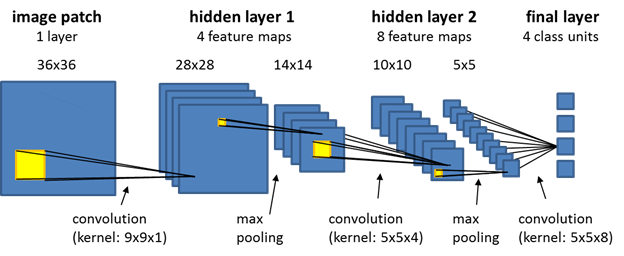
\includegraphics[width=1.0\textwidth]{matematicas/cnn_ejemplo.png}
		\caption{Ejemplo visual de una red convolucional profunda.}
	\end{figure}

\end{frame}

\subsection{Conclusiones}
\begin{frame}
	\begin{itemize}
		\item Primera conclusion
		\item Segunda conclusion
		\item Tercera conclusion
	\end{itemize}
\end{frame}
